%% This is file `elsarticle-template-1-num.tex',
%%
%% Copyright 2009 Elsevier Ltd
%%
%% This file is part of the 'Elsarticle Bundle'.
%% ---------------------------------------------
%%
%% It may be distributed under the conditions of the LaTeX Project Public
%% License, either version 1.2 of this license or (at your option) any
%% later version.  The latest version of this license is in
%%    http://www.latex-project.org/lppl.txt
%% and version 1.2 or later is part of all distributions of LaTeX
%% version 1999/12/01 or later.
%%
%% Template article for Elsevier's document class `elsarticle'
%% with numbered style bibliographic references
%%
%% $Id: elsarticle-template-1-num.tex 149 2009-10-08 05:01:15Z rishi $
%% $URL: http://lenova.river-valley.com/svn/elsbst/trunk/elsarticle-template-1-num.tex $
%%
\documentclass[preprint,12pt]{elsarticle}

%% Use the option review to obtain double line spacing
%% \documentclass[preprint,review,12pt]{elsarticle}

%% Use the options 1p,twocolumn; 3p; 3p,twocolumn; 5p; or 5p,twocolumn
%% for a journal layout:
%% \documentclass[final,1p,times]{elsarticle}
%% \documentclass[final,1p,times,twocolumn]{elsarticle}
%% \documentclass[final,3p,times]{elsarticle}
%% \documentclass[final,3p,times,twocolumn]{elsarticle}
%% \documentclass[final,5p,times]{elsarticle}
%% \documentclass[final,5p,times,twocolumn]{elsarticle}

%% The graphicx package provides the includegraphics command.
\usepackage{graphicx}
%% The amssymb package provides various useful mathematical symbols
\usepackage{amssymb}
%% The amsthm package provides extended theorem environments
%% \usepackage{amsthm}

%% The lineno packages adds line numbers. Start line numbering with
%% \begin{linenumbers}, end it with \end{linenumbers}. Or switch it on
%% for the whole article with \linenumbers after \end{frontmatter}.
\usepackage{lineno}

%% natbib.sty is loaded by default. However, natbib options can be
%% provided with \biboptions{...} command. Following options are
%% valid:

%%   round  -  round parentheses are used (default)
%%   square -  square brackets are used   [option]
%%   curly  -  curly braces are used      {option}
%%   angle  -  angle brackets are used    <option>
%%   semicolon  -  multiple citations separated by semi-colon
%%   colon  - same as semicolon, an earlier confusion
%%   comma  -  separated by comma
%%   numbers-  selects numerical citations
%%   super  -  numerical citations as superscripts
%%   sort   -  sorts multiple citations according to order in ref. list
%%   sort&compress   -  like sort, but also compresses numerical citations
%%   compress - compresses without sorting
%%
%% \biboptions{comma,round}

\newcommand{\LAPPD}{\mathrm{LAPPD^{TM}}}

% \biboptions{}

\journal{Journal Name}

\begin{document}

\begin{frontmatter}

%% Title, authors and addresses

\title{A First Characterization of a Commercial Large Area Picosecond Photodetector}

%% use the tnoteref command within \title for footnotes;
%% use the tnotetext command for the associated footnote;
%% use the fnref command within \author or \address for footnotes;
%% use the fntext command for the associated footnote;
%% use the corref command within \author for corresponding author footnotes;
%% use the cortext command for the associated footnote;
%% use the ead command for the email address,
%% and the form \ead[url] for the home page:
%%
%% \title{Title\tnoteref{label1}}
%% \tnotetext[label1]{}
%% \author{Name\corref{cor1}\fnref{label2}}
%% \ead{email address}
%% \ead[url]{home page}
%% \fntext[label2]{}
%% \cortext[cor1]{}
%% \address{Address\fnref{label3}}
%% \fntext[label3]{}


%% use optional labels to link authors explicitly to addresses:
%% \author[label1,label2]{<author name>}
%% \address[label1]{<address>}
%% \address[label2]{<address>}

\author{[ANNIE Collaboration]}

\address{Everytown, United States}

\begin{abstract}
%% Text of abstract
Here we report on the results from the testing of a first, research-grade Large Area Picosecond Photodetector (LAPPD) for the Accelerator Neutrino Neutron Interaction Experiment (ANNIE). LAPPD-25 was produced by Incom Inc and purchased by the collaboration in March 2018. Characterization was performed at a test facility at Iowa State University, featuring a blue PiLaS laser capable of up to $\sim$30 psec time resolution. Good single-photoelectron (sPE) separation was observed, with peak gain above 10$^6$. Typical sPE time resolutions of better than 70 psec were measured over the surface of the detector. Differential time resolutions of better than X psec were observed between the two ends of the transmission line anode, corresponding to spatial resolutions of x mm. 
\end{abstract}

\begin{keyword}
Science \sep Publication \sep Complicated
%% keywords here, in the form: keyword \sep keyword

%% MSC codes here, in the form: \MSC code \sep code
%% or \MSC[2008] code \sep code (2000 is the default)

\end{keyword}

\end{frontmatter}

%%
%% Start line numbering here if you want
%%
\linenumbers

%% main text
\section{Introduction}

Photodetectors~\cite{MCPref}, capable of micron-scale spatial 
resolutions~\cite{Ossy_highres2}, sub-nanosecond time 
resolutions~\cite{{timingref},{Akatsu:2004mq},{InamiRef}}, and gains exceeding $10^7$~\cite{Ossy_gain_noise_TTS}. Economical, large-area MCP photosensors with these characteristics would bring much needed timing and imaging capabilities to a wide range of applications in fields such as particle physics, nuclear physics, X-ray science, and medical imaging.

The Large Area Picosecond Photodetector (LAPPD) collaboration was formed to develop techniques for making large format (20 cm x 20 cm) MCP-PMT detector systems using scalable methods and low-cost materials, addressing technical aspects of the problem from the photocathode and the gain stage to the readout electronics and vacuum packaging. Fabrication of LAPPDs is based largely on the application of thin-film materials to glass structures. In particular, a technique known as Atomic Layer Deposition (ALD)~\cite{ALDref} enables the fabrication of large-area MCP amplification structures by conformally coating inactive, porous glass substrates~\cite{{MSDref},{fabref}}. The technique is flexible as well as scalable, allowing for the independent optimization of the 
geometric, resistive, and secondary electron emission properties~\cite{MSDref} of the channel plates.

In this paper, we present an analysis of the timing characteristics for
20 cm x 20 cm $\LAPPD$ systems.  At sufficient operational voltages, we
observe single-photoelectron time resolutions in the range of 50-60 picoseconds, consistent with those of commercial MCPs with comparable pore structures. Differential time resolutions are measured as low as 4.3 psec, with the large signal limit extrapolating below 2 picoseconds. Spatial resolutions are set by the granularity of the 
economical stripline anode design (see Sec~\ref{sec:LAPPDdesign}) 
and are measured to be less than 1 mm in both directions with respect to the stripline anodes. The median gain of the most recent MCP stack exceeds 10$^7$.


\section{The Detector}
\label{sec:Detector}

LAPPD-25 was one of the first two commercial LAPPDs sold by Incom Inc for use in research applications. The sealed tube detector was produced with a uniform gain better than 10$^6$ at operational voltages and a typical quantum efficiency of $\sim$12\%, slightly below Incom's final target value but nonetheless adequate for the ANNIE physics measurement. 

LAPPD-25 was removed from the processing chamber on January, 2018 and has been working since. These tests were conducted 3 months into its lifetime.

\section{The Facility and Experimental Setup}
\label{sec:Facility}

\noindent A new test facility was commissioned at Iowa State for the purpose of these and future measurements. Many of the fixtures and techniques used are based on prior work, described in Refs~\cite{RSI} and~\cite{8inchtiming}.\\

\noindent The ISU test facility is equipped with a large dark box, 3ft x 3ft x 6ft, instrumented with patch panels containing HV, BNC, SMA, USB, and LEMO feedthroughs.\\


%\begin{figure}
%	\centering
%	 \begin{tabular}{c c}
%                \includegraphics[width=0.55\linewidth]{plots/IMG_7105.jpg}&
%                \includegraphics[width=0.31\linewidth]{plots/IMG_7103.jpg}\\
%         \end{tabular}         
%	\caption{LEFT: A picture of the ISU dark box. RIGHT: Close up showing the new SMA/USB patch panel.}
%	\label{fig:darkbox}
%\end{figure}

\noindent The primary light source at the ISU test stand is a blue (405 nm) PLAS laser with $\sim$30 psec resolution. The laser pulses are injected into a single-mode fiber optic for delivery to the LAPPD. At the outgoing collimation optic is cage plate with neutral density filters used to attenuate the laser to single photoelectron (sPE) light intensities. A motorized 2-D stage is used to deliver the outgoing light from the fiber and can be remotely controlled from outside the darkbox with micron-level precision.\\

\noindent Three high voltage supplies were used to control the voltages of the LAPPD. One supply was connected to the photocathode. The second supply was connected to the top of the MCP closes to the photocathode, and the third supply was connected to the bottom of the same MCP. A voltage divider connected the bottom of the topmost MCP to the top of the second MCP and the bottom of the second MCP to ground. This configuration is shown in Fig~XX. For the rest of this paper, the three operational voltages will be specified in order from the photocathode towards ground. We will also specify the effective voltages across each MCP and gap, calculated based on the known resistances of the two MCPs.\\



%\begin{figure}
%	\centering
%               \includegraphics[width=0.75\linewidth]{plots/IMG_7087.jpg}	
%	\caption{The fully assembled breadboard containing LAPPD-9 with all RF and HV connections, and the mounted laser optics.}
%	\label{fig:breadboard}
%\end{figure}


\section{Measurement Strategy}
\label{sec:Method}

\noindent A pulsed, sub-ps laser was used to characterize the time resolution of the large-area MCPs. Absolute timing of the MCP response was measured in relation to a fast photodiode triggered by the laser. Single-photoelectron operation was achieved by controlling photon statistics.\\

\noindent The average 405nm laser power, of order 100 nano-Watts, was sufficient to produce many photoelectrons per pulse, even with a low quantum efficiency (QE) aluminum photocathode. Without attenuation, the fraction of laser pulses with an observed MCP signal was 100\%. However, the beam could be attenuated to the point where some fraction of laser pulses produced no discernible signal, as determined from the oscilloscope data using analysis techniques described in Ref~\cite{RSI}. Once the detector was operating in a regime where the fraction of events with good pulses was sufficiently low, the probability of producing more than one PE was statistically suppressed. Fig. 5 shows the relationship between average UV intensity and the probability of an MCP signal. The slope of this plot at low laser intensities can be used to extrapolate to higher intensities, providing a statistical handle on the number of photoelectrons. This approach does not depend on the choice of photocathode or precise knowledge of the QE.\\


%\section{Measurement History}
%\label{sec:Method}

%\noindent Maybe not needed....

\section{Reconstruction Strategy}
\label{sec:Reco}

\noindent For this first study, we use simple CFD-based algorithms for reconstructing pulse times. These data will be soon reanylzed using a full template-based shape fit method. Nonetheless, for single-PE timing the algorithms presented here should suffice. \noindent FFT filtering was applied to remove high frequency and low frequency noise, as well as filtering out specific 88.5 MHz noise from the local college radio station  (see Fig~\ref{fig:FFTandCFD}). Pulse candidates are selected using a time-above-threshold cut, which can identify even signals with a peak amplitude within the electronics noise. Pulses were required to provide a sustained signal above 0.4 mV for over 1.5 nsec. Once identified, the arrival time of the pulses was determined using a simple Constant Fraction Discriminator (CFD) algorithm. Pulses were added to their inverse, multiplied by a fraction (in this analysis 50\%) and shifted by a fixed phase (in this analysis 1 $\mu$sec). The arrival time is defined as the point where the resulting shape first crosses the time axis. For studying the gain of the detector and single PE transit time spread (TTS) we look for pulses on a single strip where there are no signals on the neighboring channels. We observed that the majority of pulse candidates (more than 90\%) were localized on a single strip.\\

%\begin{figure}
%	\centering
%	 \begin{tabular}{c c}
%                \includegraphics[width=0.48\linewidth]{plots/Example_FFT1}&
%                \includegraphics[width=0.48\linewidth]{plots/CFD_example}\\
%         \end{tabular}         
%	\caption{LEFT: The raw signal from LAPPD-9 (red) compared with the shape after high frequency noise and the 88.5 MHz background is filtered (blue). RIGHT: The fitted shape from the CFD algorithm. The arrival time of the signal is defined as the first zero-crossing of this curve.}
%	\label{fig:FFTandCFD}
%\end{figure}

\section{Results}
\label{sec:Results}

\noindent First we looked at the dark rates on a sampling of striplines accross the MCP.  Rates varried from channel to channel, from tens of Hz to hundreds of Hz. Most of the data taken for this measurent was collected in the neighborhood of a low-noise cluster of striplines: 14, 15, and 16 counting from xx.\\

\subsection{Typical Pulse Characteristics}

\begin{figure}[h]
	\centering
       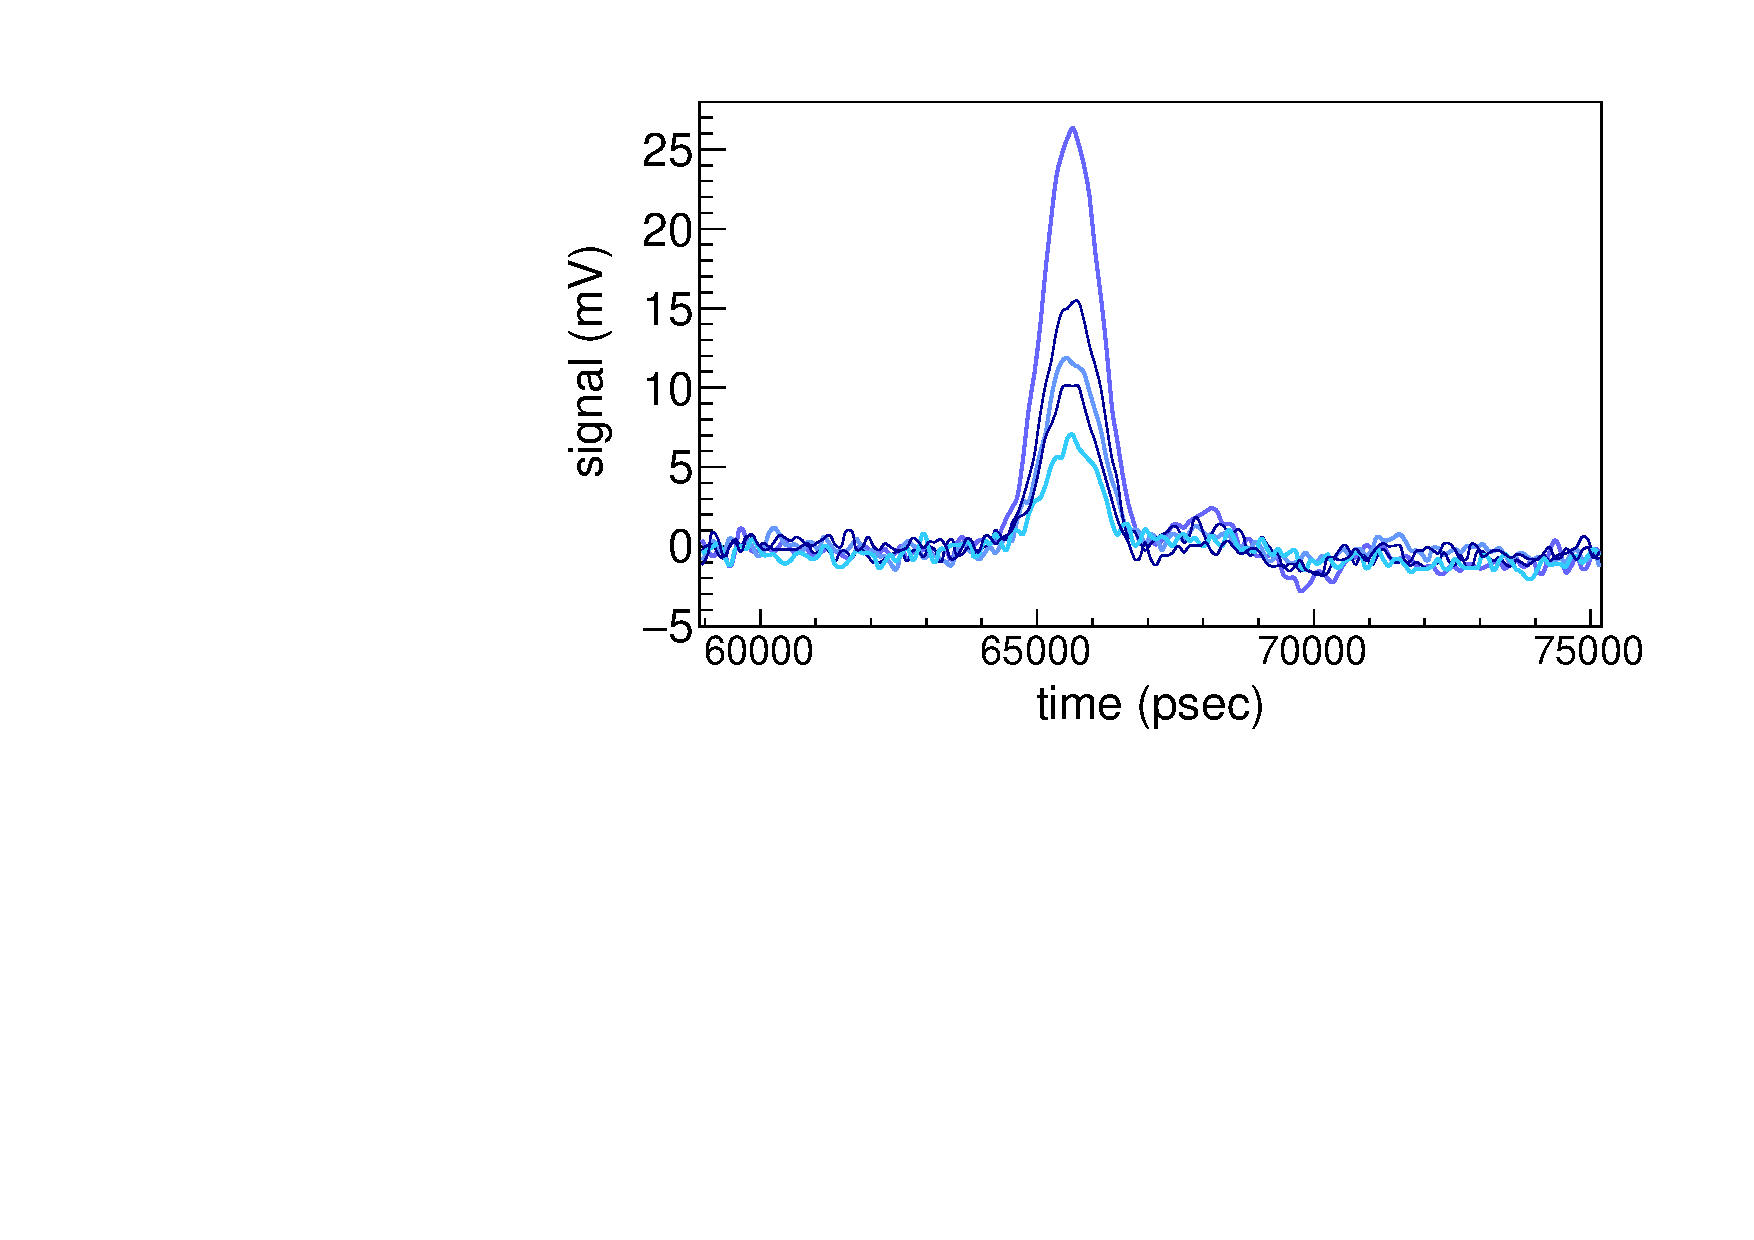
\includegraphics[width=0.75 \linewidth]{plots/TypicalPulses}
       \caption{A sampling of typical pulses on LAPPD 25. The pulses have a rise time of 850 picoseconds, and a Full Width at Half Max (FWHM) of 1.1 nanoseconds.}
	\label{fig:typicalpulses}
\end{figure}

Figure~\ref{fig:typicalpulses} shows a few randomly chosen pulses from LAPPD-25. The rise time of the pulses is roughly 850 picoseconds, and a full width at half max (FWHM) of roughly 1.1 nanoseconds. Figure XX shows the Fourier spectrum of a typical pulse, compared with that of the noise. 

\subsection{Amplitude, Gain, and Gain Uniformity}

Figure~\ref{fig:amp} shows the amplitude distribution for pulses at our nominal operational voltages of xx-yy-zz. 

\begin{figure}
	\centering
        \begin{tabular}{l l}
                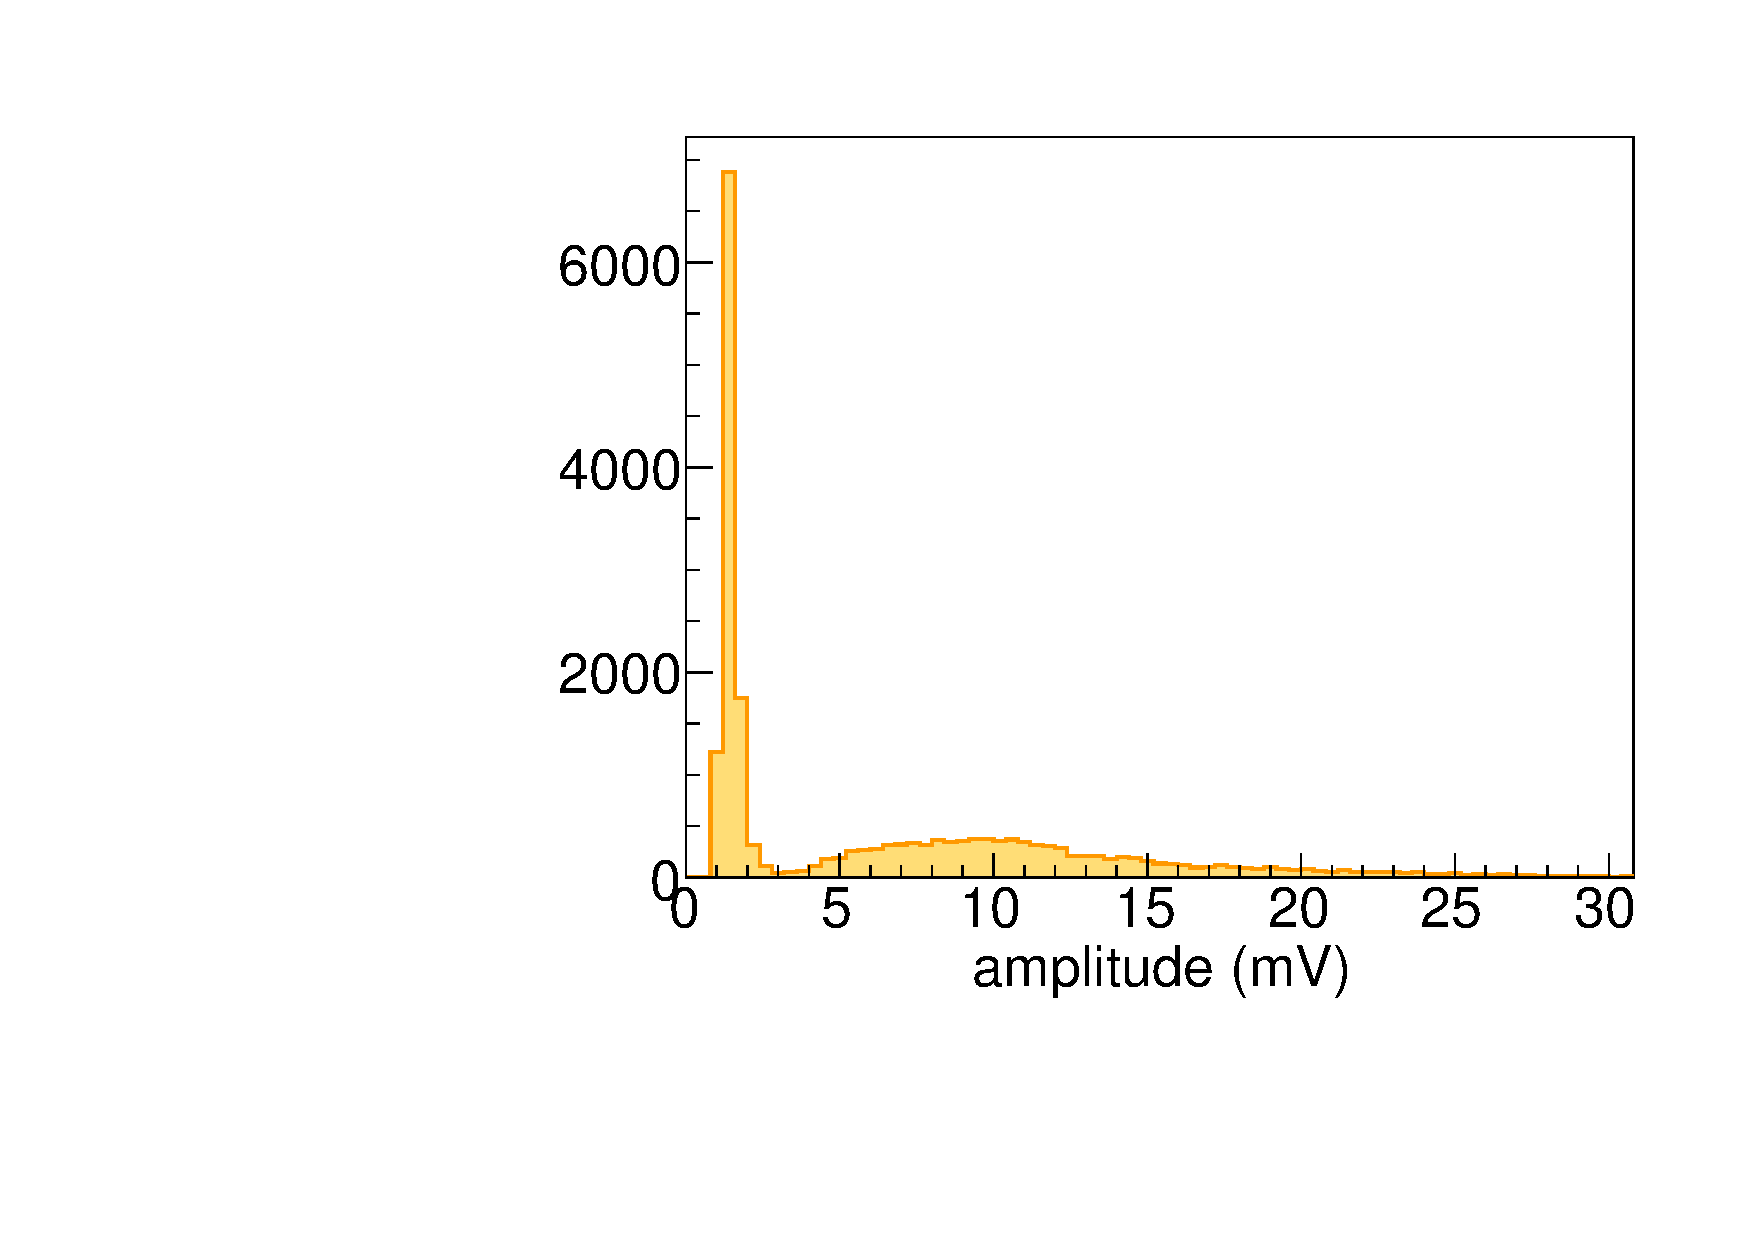
\includegraphics[width=0.52\linewidth]{plots/Amplitudes_notlog} &
                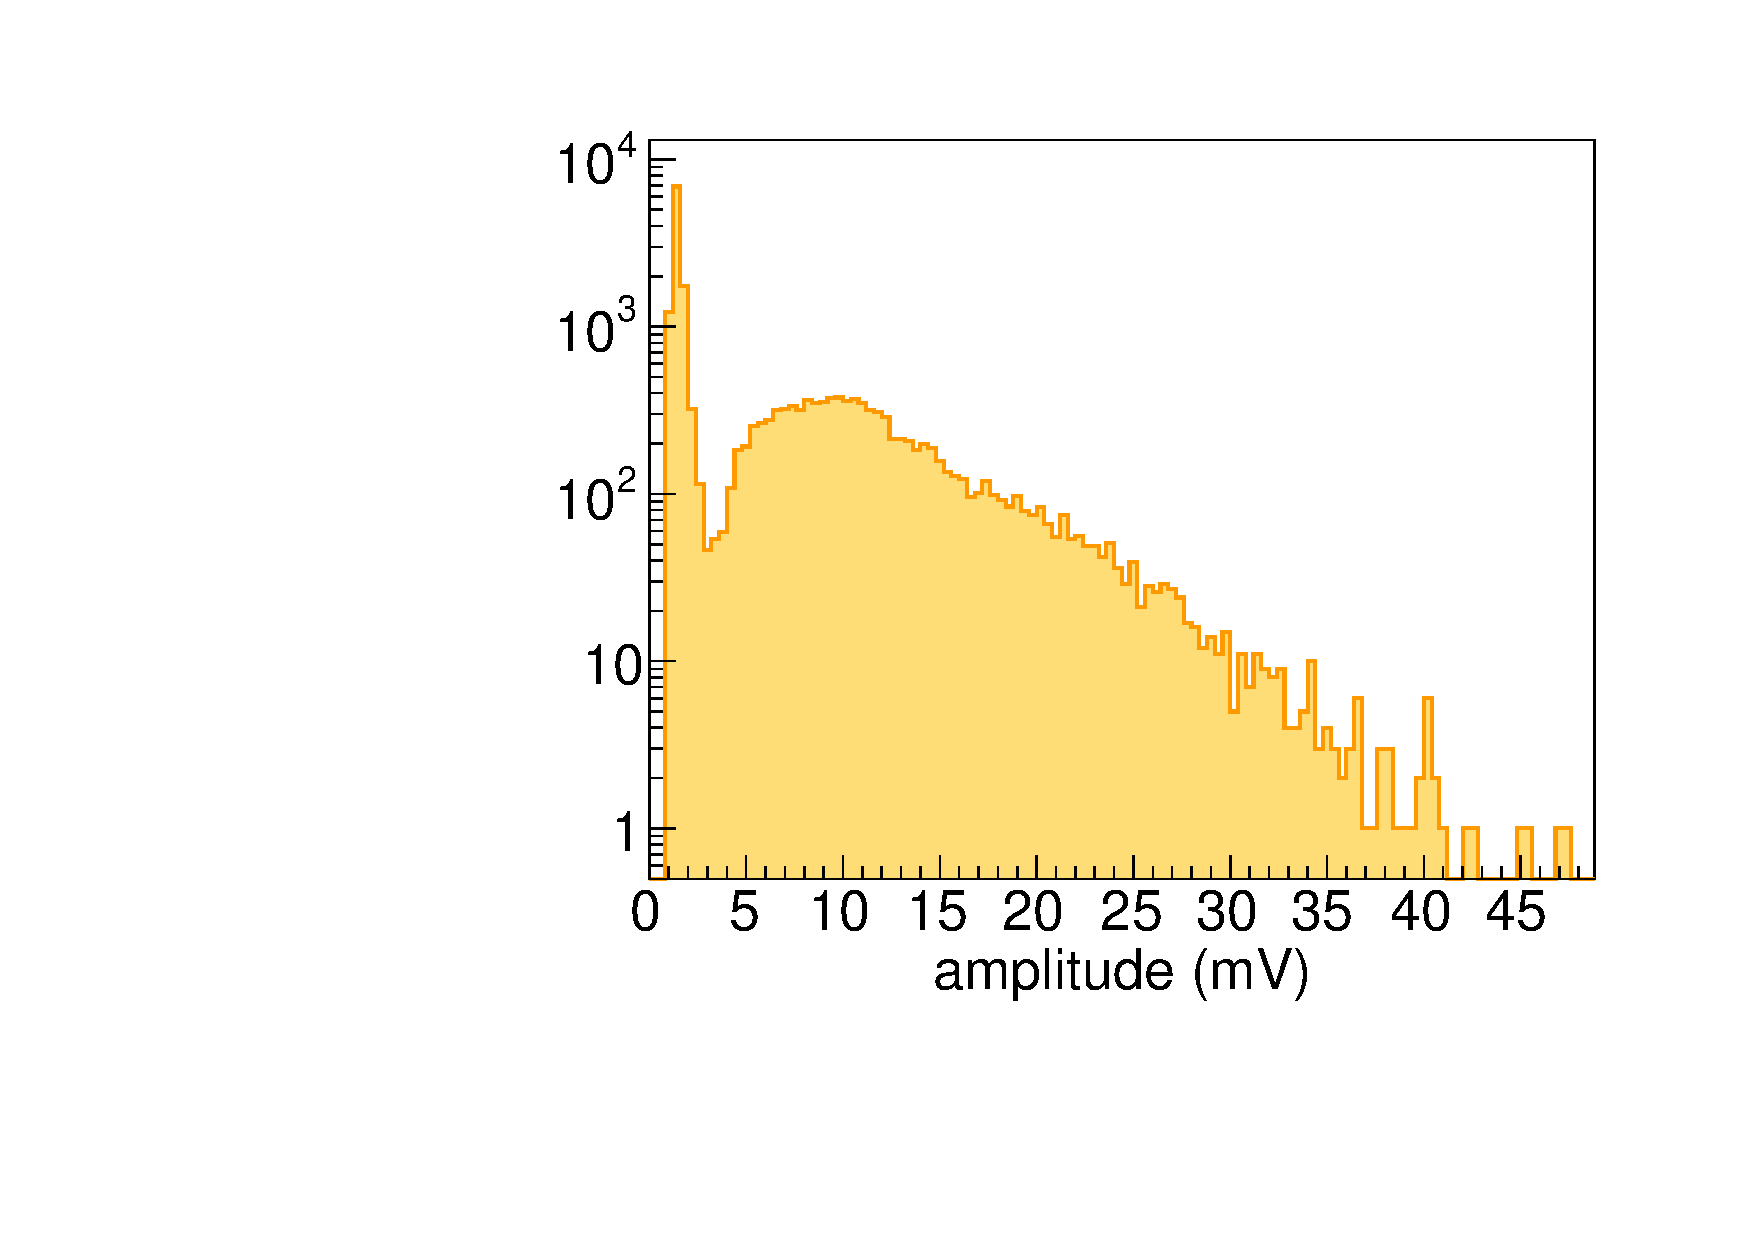
\includegraphics[width=0.53\linewidth]{plots/Amplitudes}\\
         \end{tabular}  
       \caption{The amplitude distribution for pulses on a single-side of a stripline anode.}
	\label{fig:amp}
\end{figure}

\begin{figure}
	\centering
       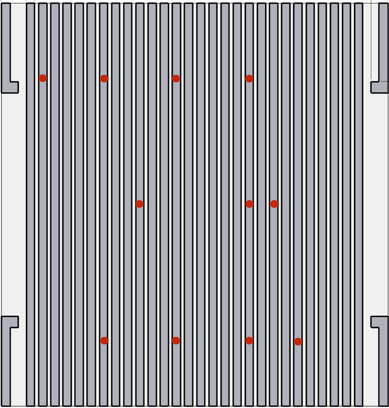
\includegraphics[angle=90, width=0.45\linewidth]{plots/positions}  
       \caption{The laser positions used for the spatial uniformity scan with respect to the anode pattern. These laser positions are identified by their strip number (counting up from one) and on which side of the strip the laser was located (L=left, C=center, R=right)}
	\label{fig:positions}
\end{figure}

\begin{figure}
	\centering
        \begin{tabular}{l l}
                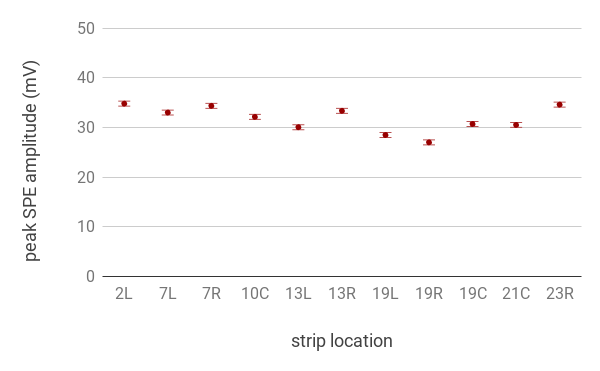
\includegraphics[width=0.48\linewidth]{plots/SinglePEAmplitudePeak_notitle} &
                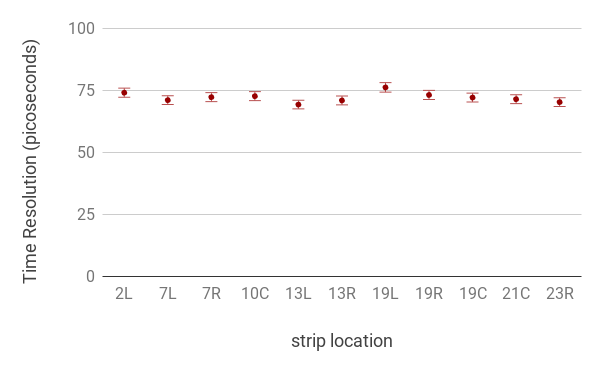
\includegraphics[width=0.48\linewidth]{plots/SinglePETimeResolution_notitle}\\
         \end{tabular}  
       \caption{LEFT: Variation in the fitted single PE peak amplitude for data collected at each of the 11 positions on LAPPD-25 shown in Fig~\ref{fig:positions}. RIGHT: Variation in the fitted time resolution of the main peak of the transit time spread distribution for the same 11 positions.}
	\label{fig:amp}
\end{figure}


\subsection{Time Resolution}


\subsection{Parallel Scan}


\begin{figure}
	\centering
        \begin{tabular}{l}
                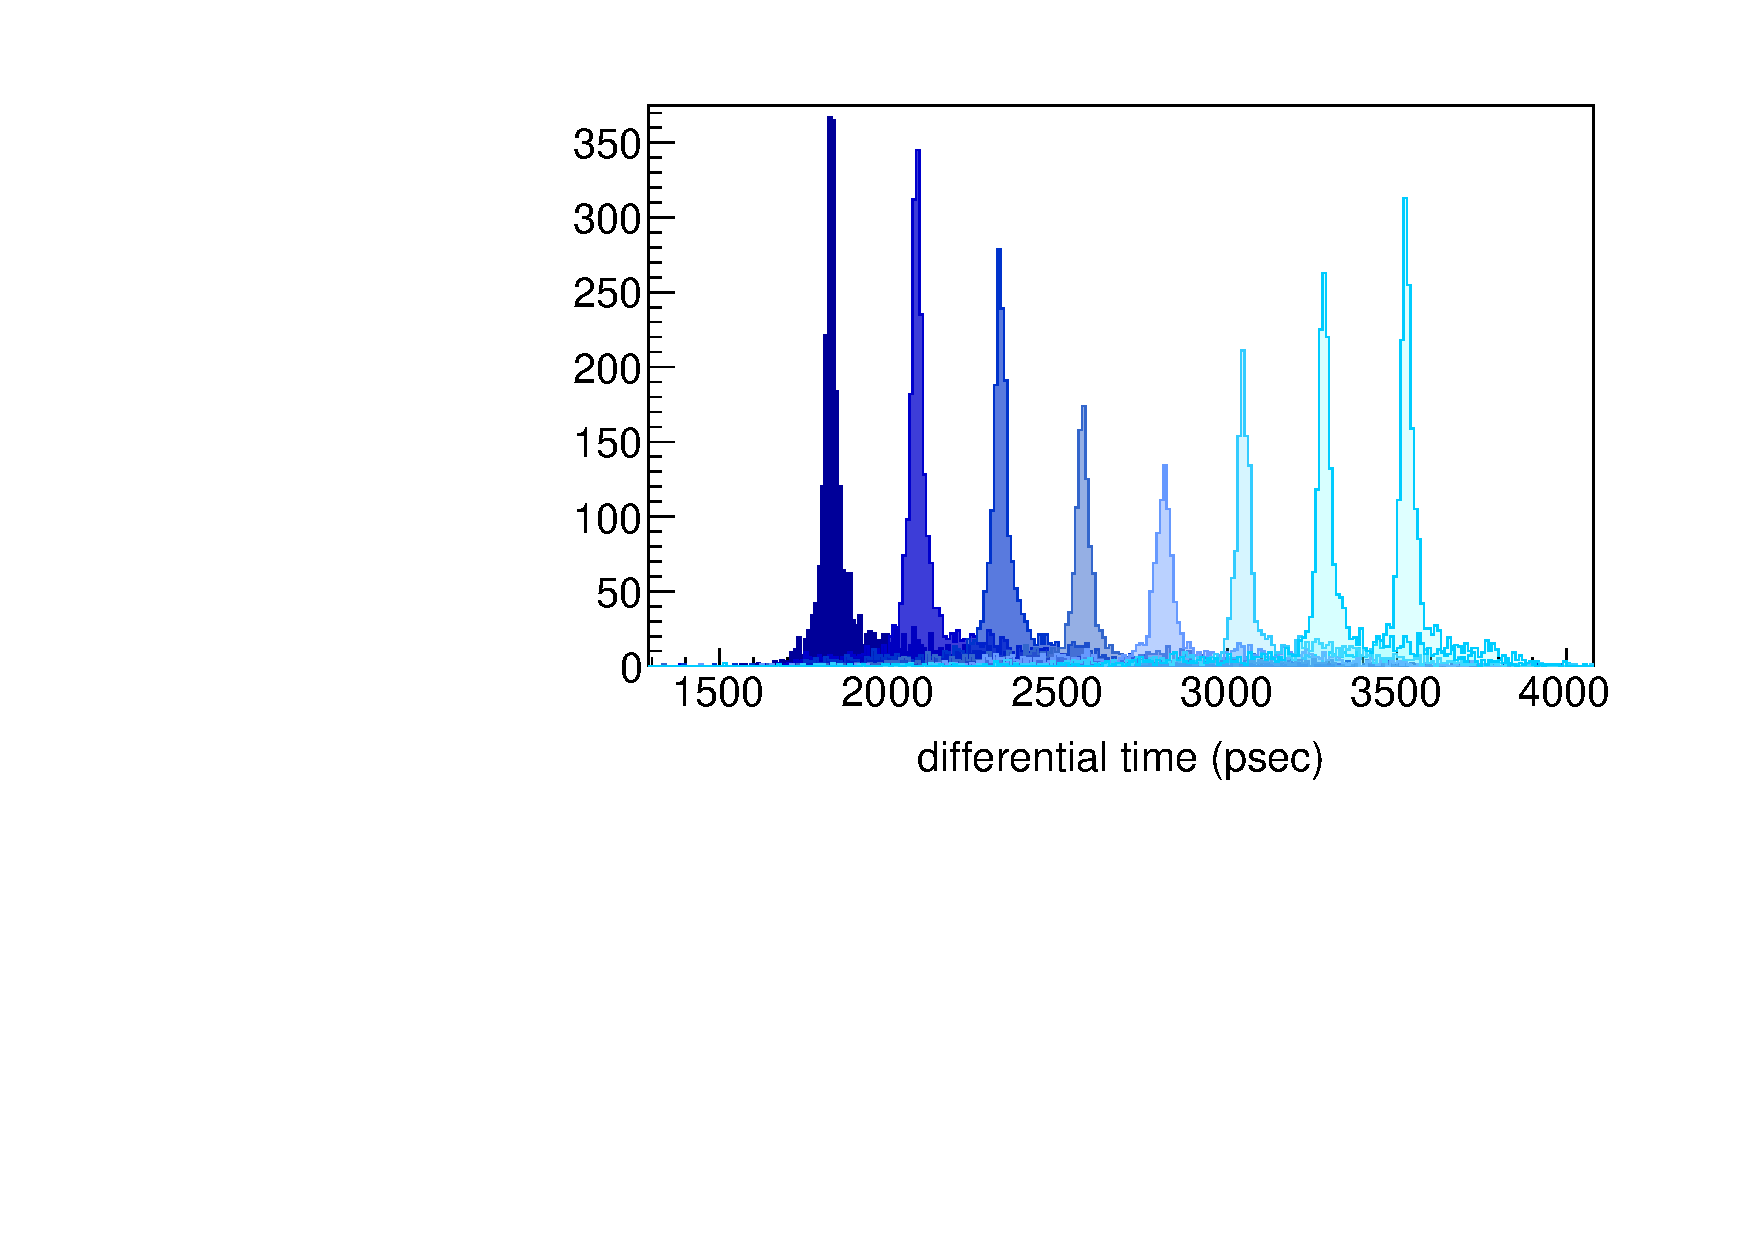
\includegraphics[width=0.6\linewidth]{plots/difftime} \\
                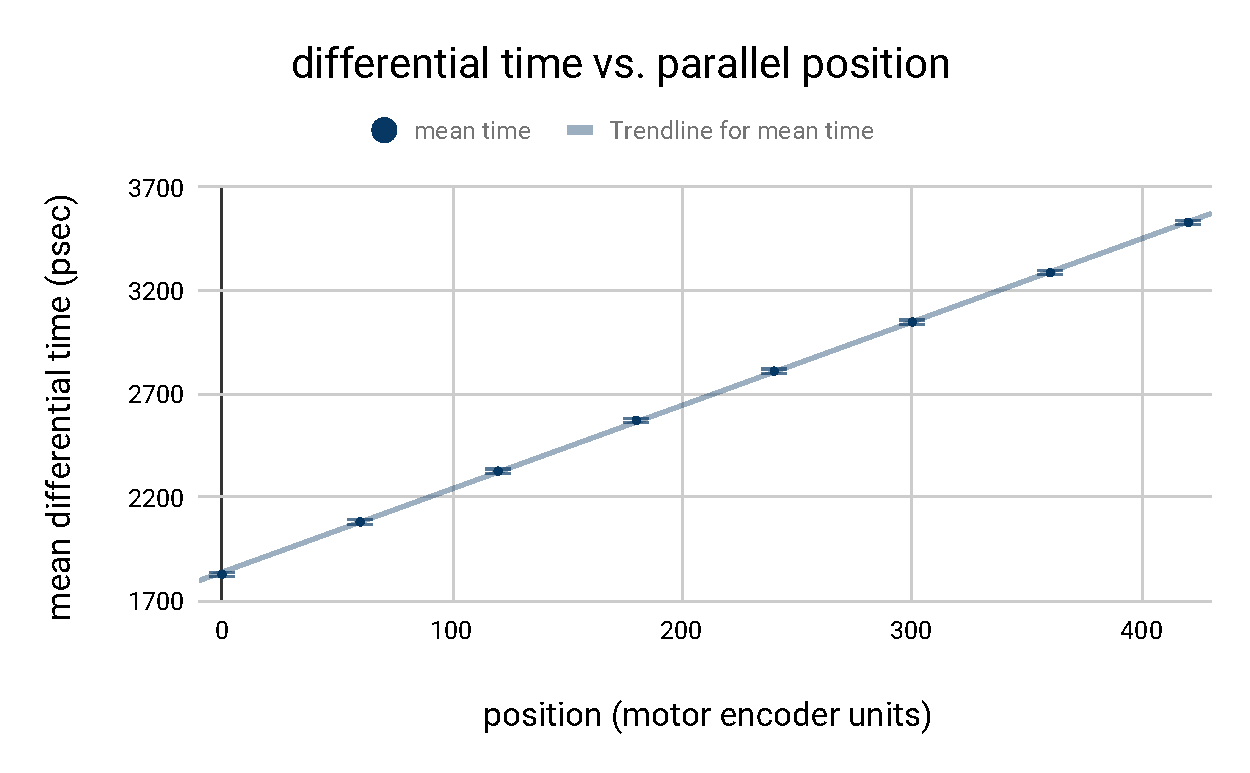
\includegraphics[width=0.55
            \linewidth]{plots/differentialtimevsparallelposition}
         \end{tabular}  
       \caption{TOP: The differential timing distributions for each position taken during the parallel scan. BOTTOM: Fitted mean differential time as a function of position (10x errors) with a linear regression.}
	\label{fig:amp}
\end{figure}


\subsection{After Pulsing}

\subsection{Dark Rates}

\noindent Signals produced by LAPPD-9 in single-PE mode were very small, just distinguishable above noise on the channel. This made identification of pulses difficult and reduced the time resolving capabilities. Figure~\ref{fig:examplesPEpulses} shows some typical single-PE pulses observed from the detector. Figure~\ref{fig:ssignoise}, on the left, shows the distibution of noise on a typical baseline of our signal channel, with a fitted sigma of roughly 0.2 mV. The plot on the right overlays this noise with the distribution of signal-pulse amplitudes (abitrary normalization of the two distributions). Figure~\ref{fig:sPEPHD} shows the gain distribution for single PE pulses produced in the detector. The gains of some pulses  were as high as 10$^6$, but more of the peak of the distribution looks to be in the high 10$^4$ range, making efficient photon counting difficult.

\noindent Figure~\ref{fig:sPETTS} shows the single PE transit time spread taken at one point on the detector. The sigma of the fitted Gaussian is 314 picoseconds, which is larger than the $\sim$50 psec limit for 20 micron MCPs. However, given the signal to noise of typical single-PE pulses, this result is consistent with expectations for small signals. The time resolution can be estimated using a parameterization described by S. Ritt in Reference~\cite{Ritt}. This formula is shown. shown in Equation~\ref{eq:signal}. Given signal-to-noise ratios of 4:1 and a 300 MHz, 10 GS/sec oscilloscope, we would expect to achieve at best 150 picosecond time resolution. Using a simple CFD algorithm and not exploiting the shape of the waveforms, 300 psec is not unreasonable. Jitter in the photodiode response contributes slightly to the measured TTS, but it is small compared the resolution of the LAPPD itself. We expect with larger signals, either from more light or from future higher-gain prototypes, the resolution should get better. Indeed, Fig~\ref{fig:largesigTTS} shows a time resolution of around 65 psec for data with an arbitrarily larger number of PEs per pulse.

\begin{equation}
\Delta t = \frac{\Delta u}{U} \times \frac{1}{\sqrt{3f_s \times f_{3dB}}}
\label{eq:signal}
\end{equation}






\begin{figure}
	\centering
        \begin{tabular}{l l}
                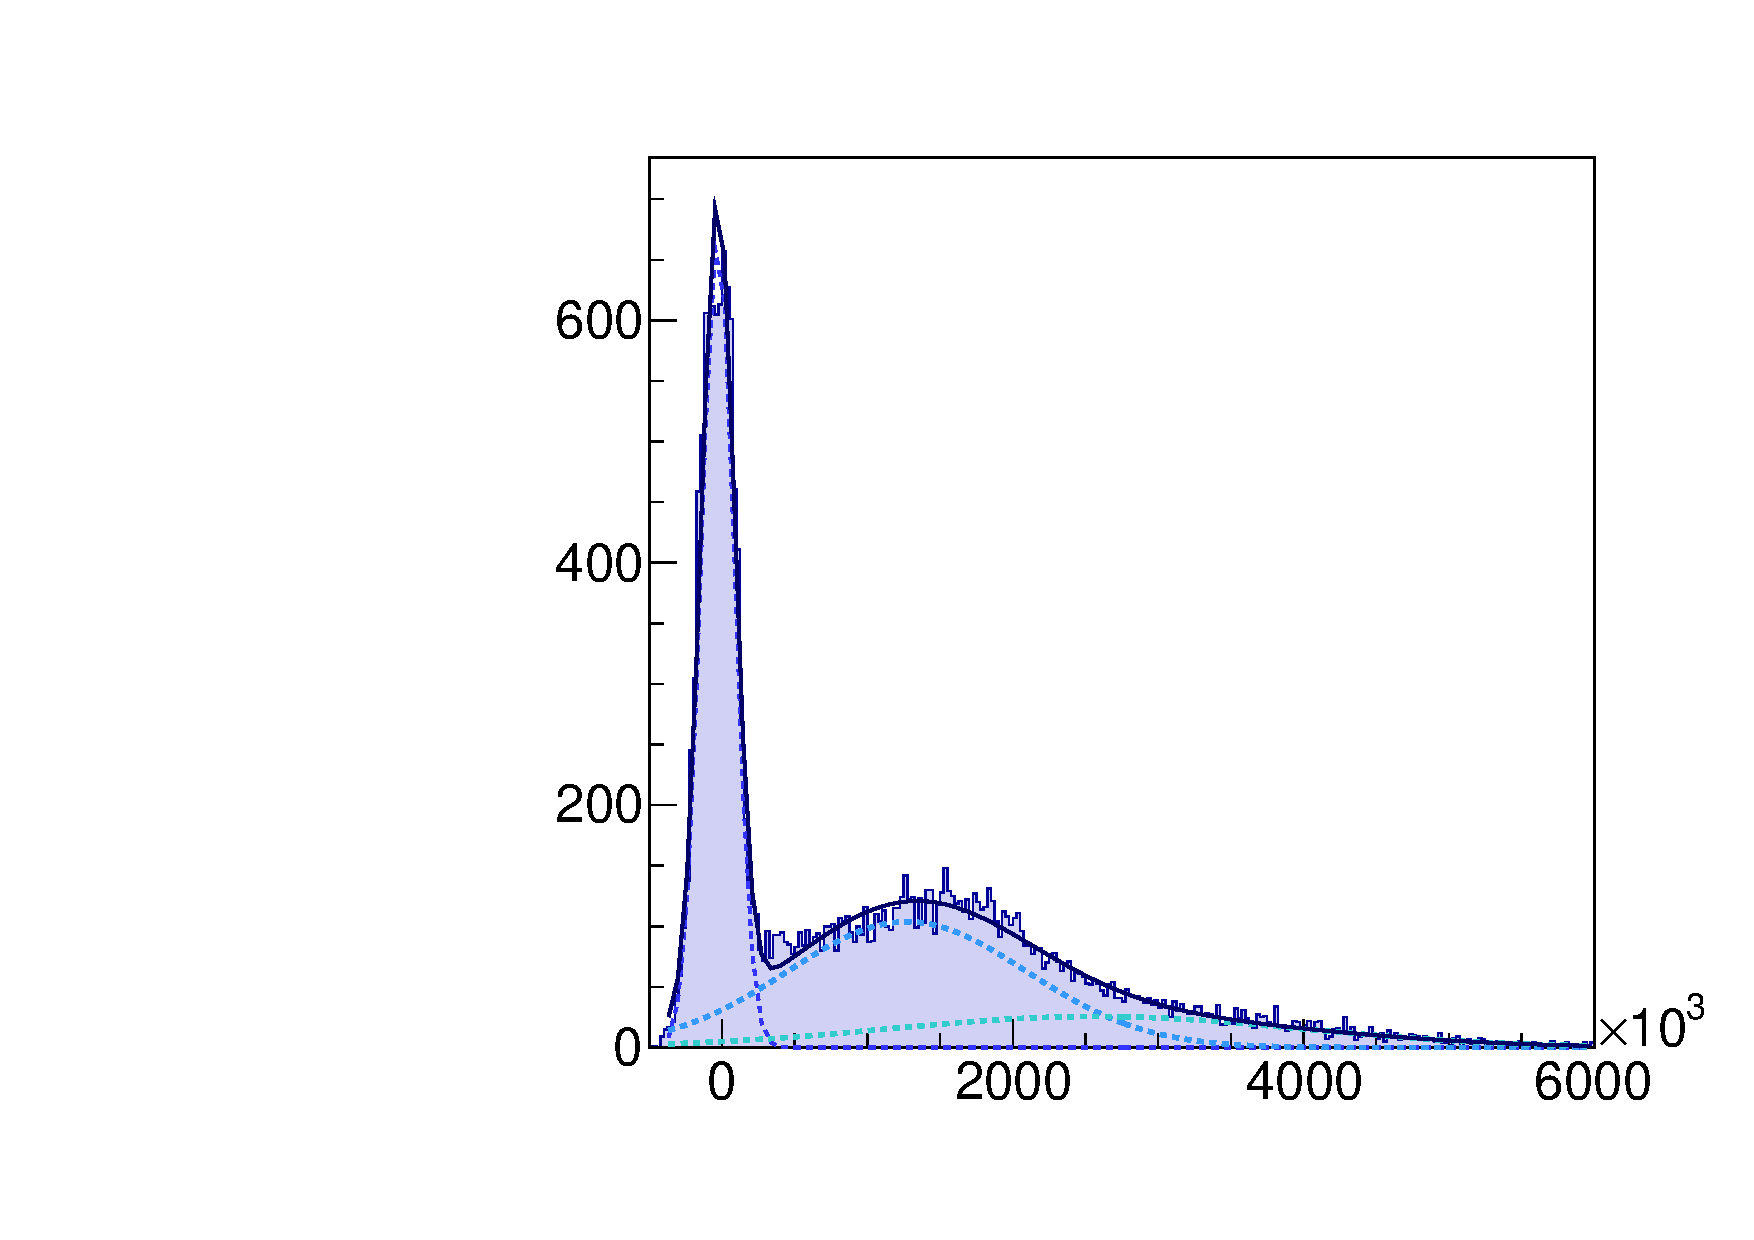
\includegraphics[width=0.42\linewidth]{plots/PulseHeightDist_notlog} &
                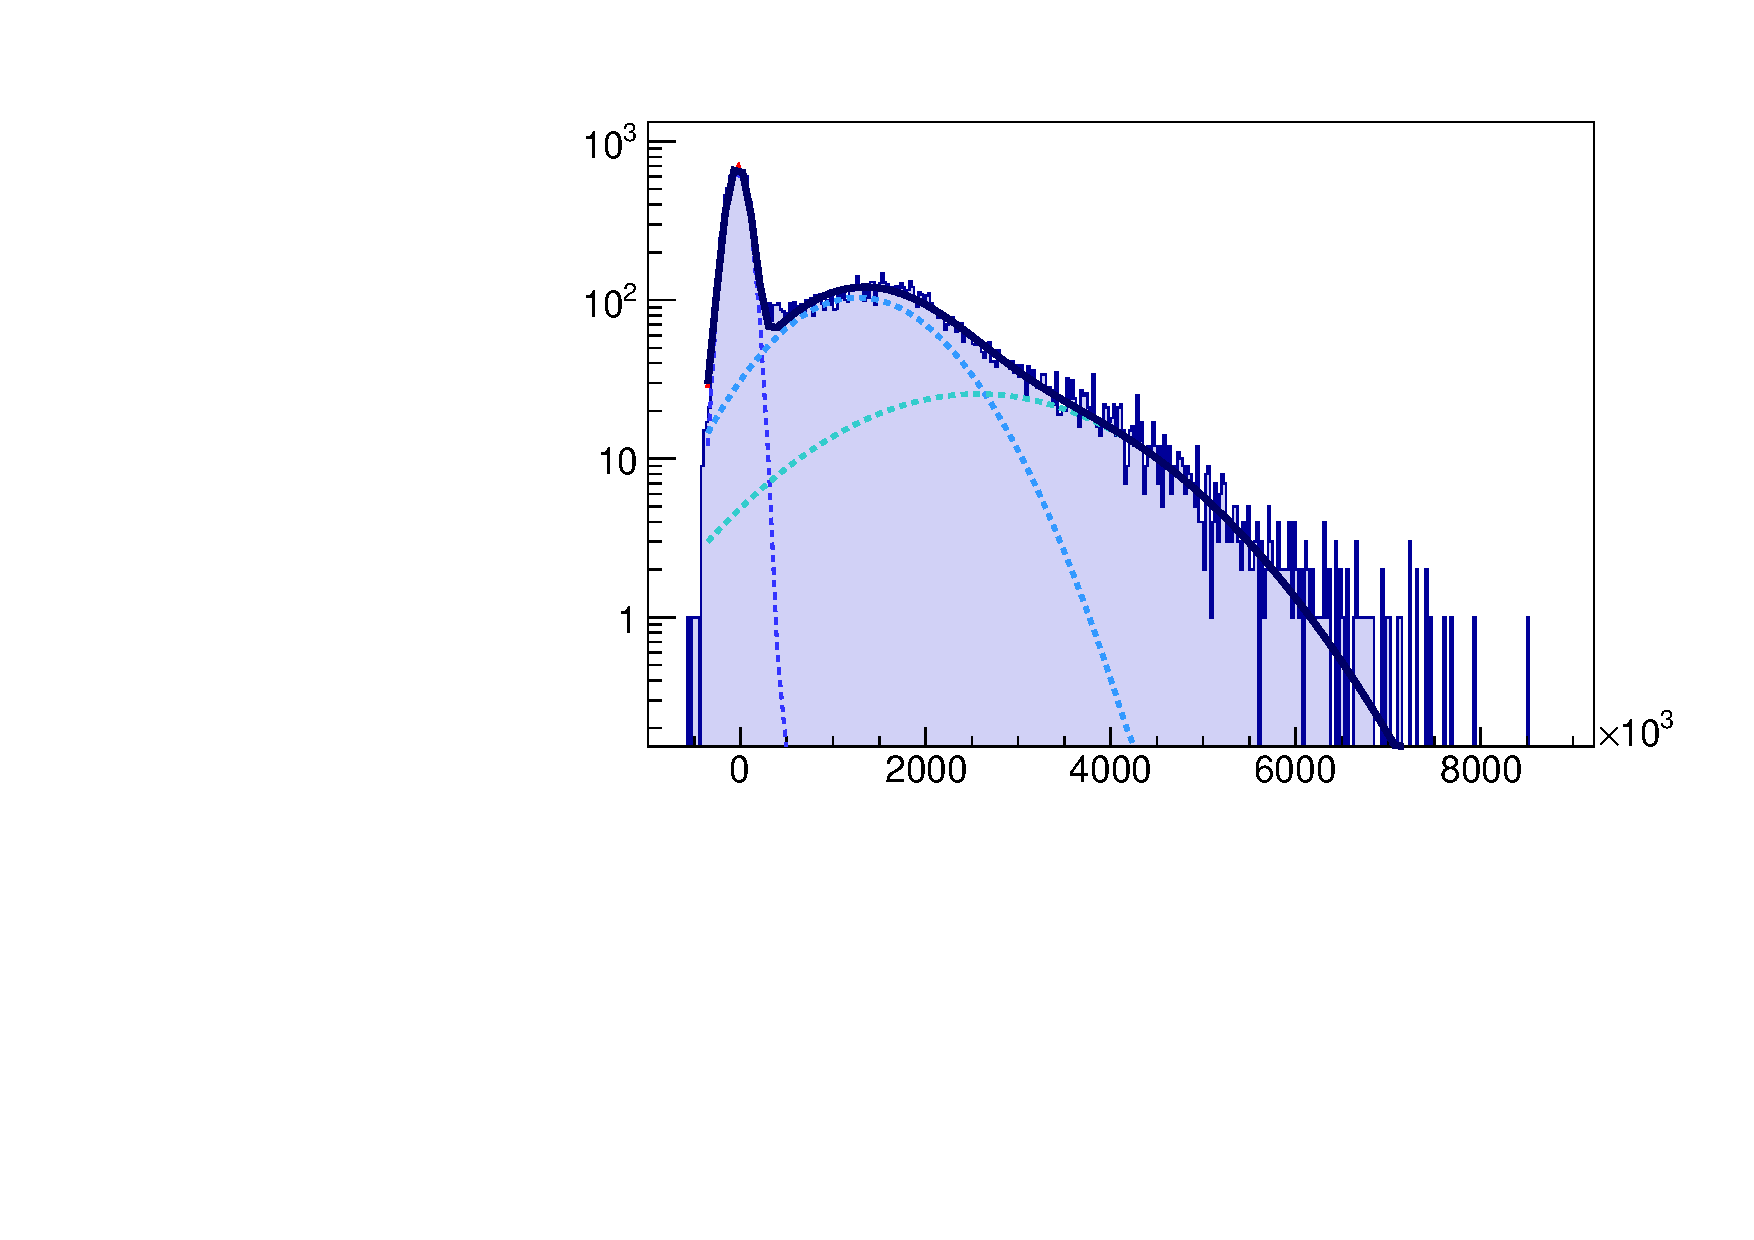
\includegraphics[width=0.57\linewidth]{plots/PulseHeightDist_log}\\
         \end{tabular}  
       \caption{A typical pulse height distribution on linear scale (LEFT) and log-scale (RIGHT) for LAPPD 25 operated at the nominal high voltages used in this paper (350,800,200,950,200)V. The single PE peak corresponds to a gain of 2.54x10$^6$ for total total charge on both sides of the stripline.}
	\label{fig:crossbar}
\end{figure}


\begin{figure}
	\centering
        \begin{tabular}{l l}
                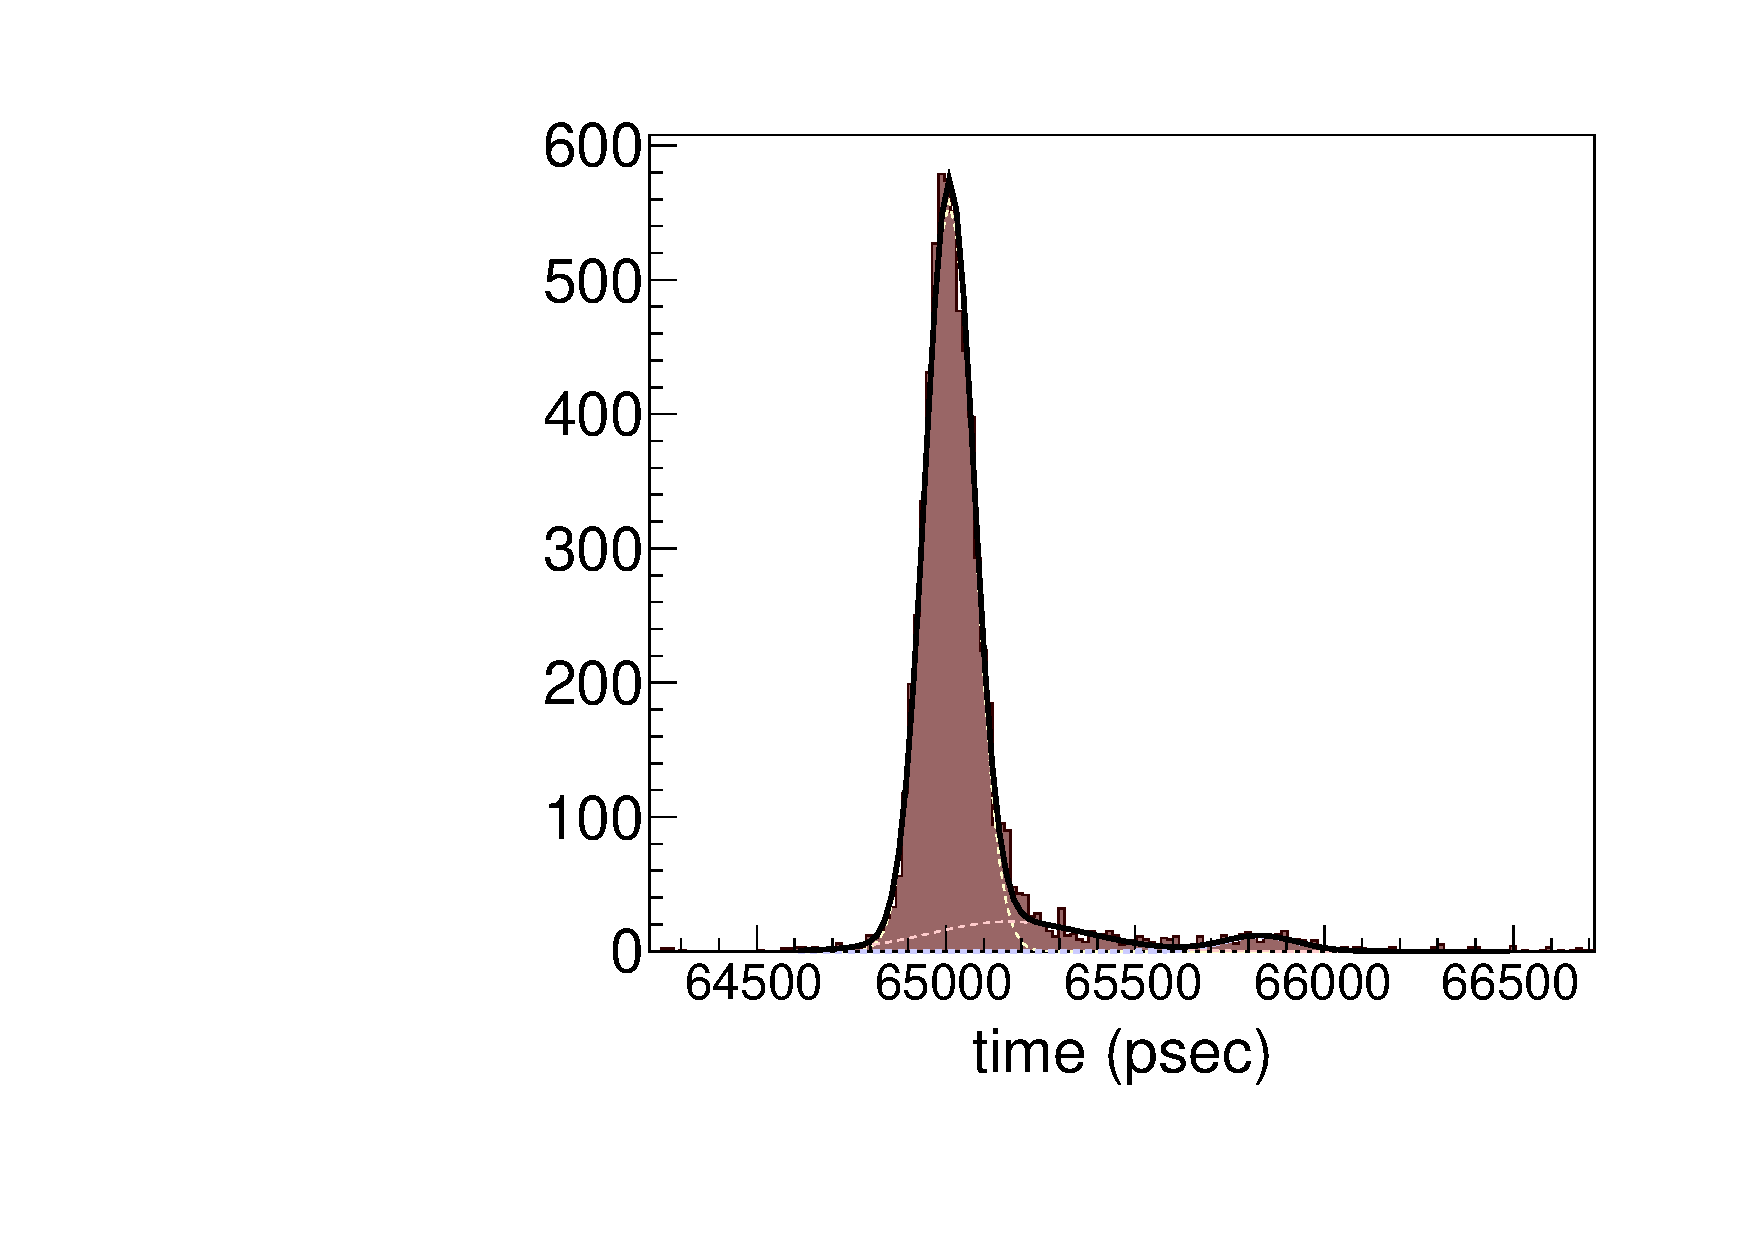
\includegraphics[width=0.42\linewidth]{plots/TTS_notlog} &
                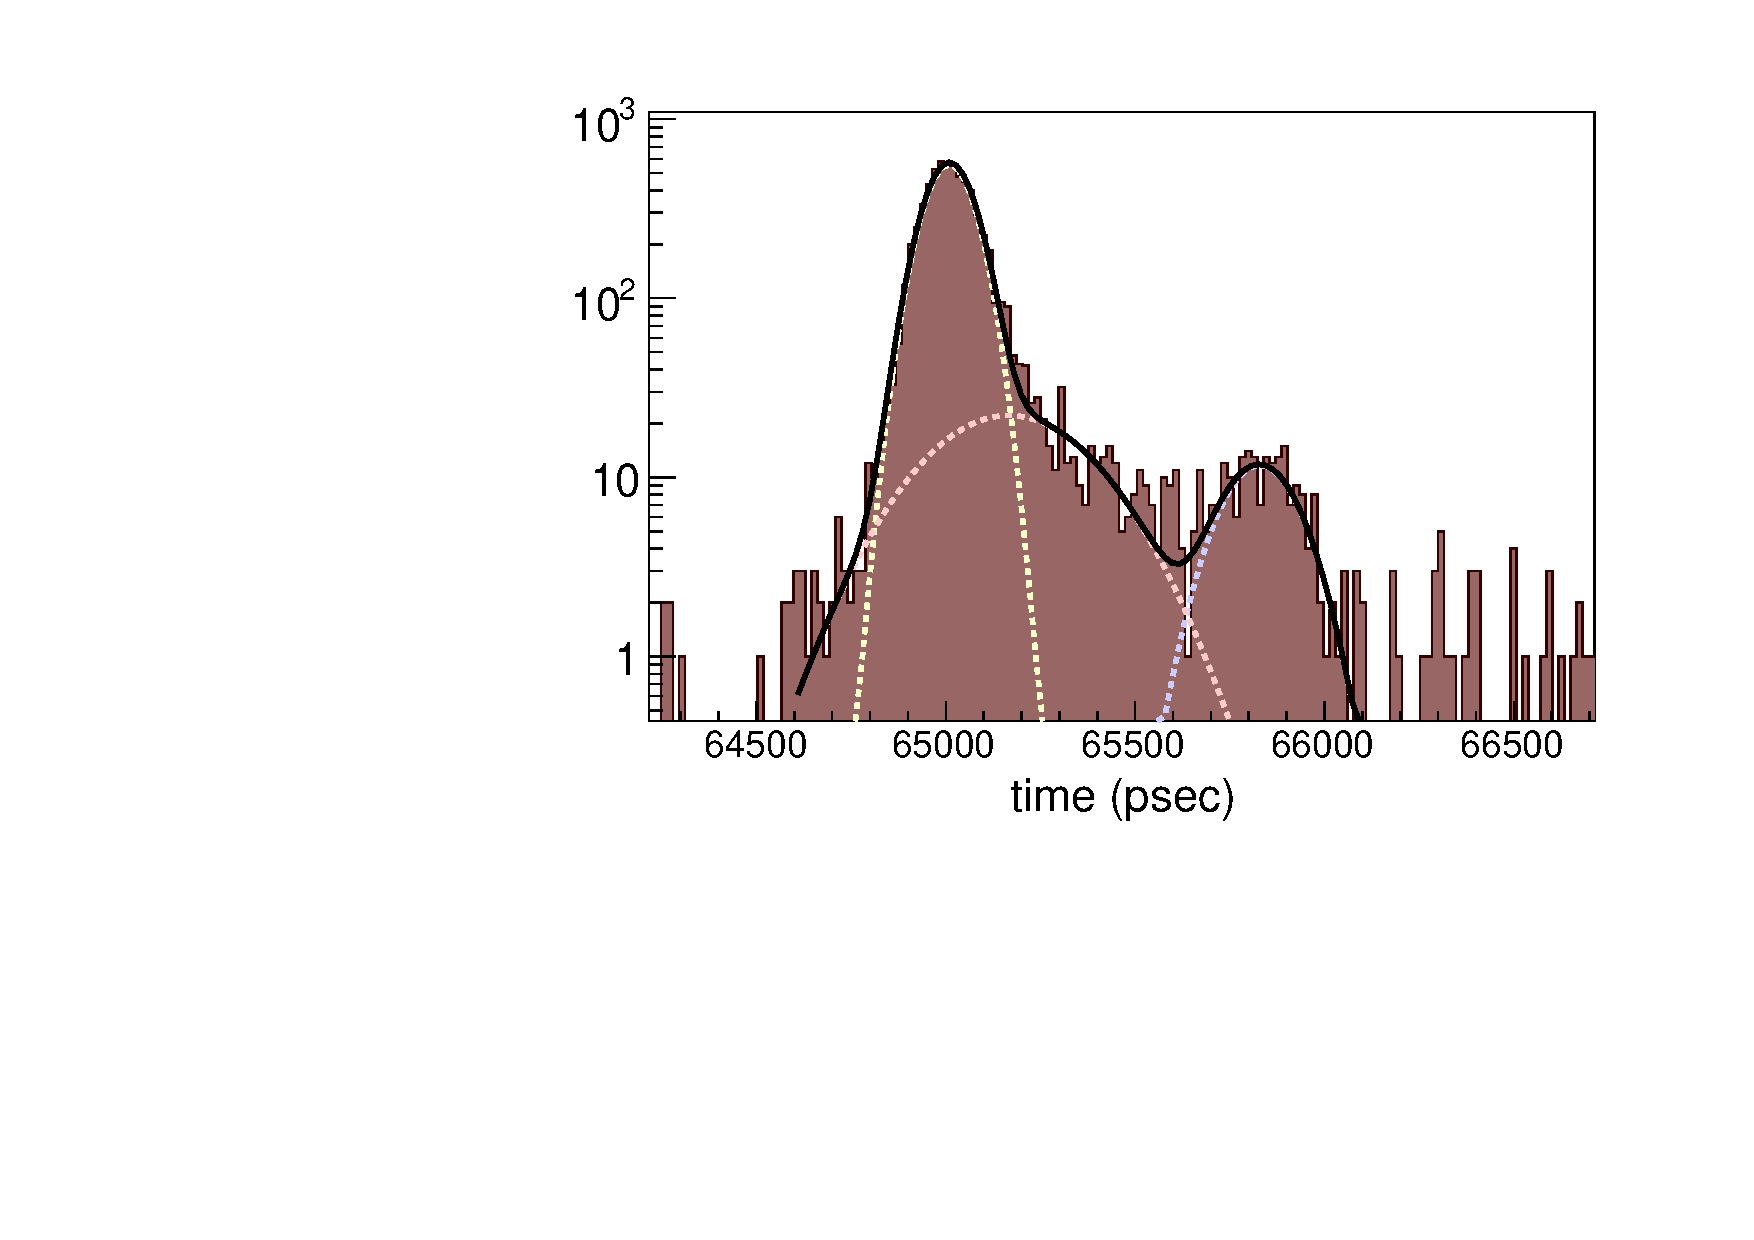
\includegraphics[width=0.56\linewidth]{plots/TTS_log}\\
         \end{tabular}  
       \caption{A typical transit time spread (TTS) on linear scale (LEFT) and log-scale (RIGHT) for LAPPD 25 operated at the nominal high voltages used in this paper (350,800,200,950,200)V. The distribution is fit with three gausians.}
	\label{fig:crossbar}
\end{figure}


%\noindent Figure~\ref{} shows the result of the parallel scan using the pen-ray lamp. The x-axis shows the position of the holes relative to pinhole-0 in centimeters, while the y-axis plots the differential time between the signals arriving at both ends of stripline-15. 

%\begin{figure}
%	\centering
%                \includegraphics[width=0.85\linewidth]{plots/m1-0_4chan_plots/Example_singlePE_pulses}
%	\caption{Some examples of single PE pulses for operation at 3200V on the photocathode and 1650V on the top of MCP2.}
%	\label{fig:examplesPEpulses}
%\end{figure}

%\begin{figure}
%	\centering
%	 \begin{tabular}{l l}
%                \includegraphics[width=0.45\linewidth]{plots/NoiseP16}&
%                \includegraphics[width=0.45\linewidth]{plots/BaselineAndSig}\\
%         \end{tabular}         
%	\caption{LEFT: The distribution of noise on the scope channel. RIGHT: The amplitudes of candidate signals overlaid on the noise distribution (arbitrary normalization).}
%	\label{fig:ssignoise}
%\end{figure}






%\begin{equation}
%\nu_{\mu} n \rightarrow \mu^{-}p\pi^{0} \rightarrow \mu^{-}ppp 
%\end{equation}



\section{Lessons Learned and Future Plans}
\label{sec:Lessons}

\noindent A number of lessons were learned in the implementation of these tests that will lead to improvements for future characterization. With only two active high voltage supplies, we were forced to make a passive divider to distribute one of the HV power supplies between the photocathode, top, and bottom of the entry-MCP, and one to divide between the top and bottom of the exit-MCP. Consequently, we did not have fine control with which to optimize the voltages. To address this in future measurements, Bernhard is developing a 5 channel system, built around EMCO power cubes. The G10 bars used to make RF and HV connections will also be improved. Groves are to be cut into the bar following the spacing of the anode patter and better methods used to attach the RF fingers. Supports will be place on the top of the dark box to help organize and manage cabling. This will also help to mitigate the 88.5 MHz interference from the ISU radio station, which is wost when there are loops of signal cables. Based on drawings made during the assembly, we also plan to make better optical mounts for the laser optics.\\

\noindent A major challenge discovered during the testing of LAPPD-9  was the interference caused by scattered laser light bouncing around in the dark box. In our final design, a barrier with a small hole was placed between the laser and the portion of the dark-box with the photodetector. Work to futher improve this aspect of the set-up is ongoing.\\

\noindent Upcoming tests of LAPPDs with multi-alkai photocathodes will rely heavily on the ISU-Neutrino Group's blue PLaS laser. Starting from a more complete system, it will be faster to move from setting up the detector to testing. We anticipate being able to collect much more data, scanning over many more voltages and positions. We are also working on integration of the PSEC electronics to be used in ANNIE. In the spring we will be ready and willing to do some lifetime testing, operating the LAPPD as part of a Cherenkov-based cosmic tracker and used in the ANNIE vertical integration testing.\\

\section{Conclusion}
\label{sec:Conclusion}

\noindent First tests of LAPPD-9 were largely successful. Nearly 5 months since its fabrication, we were able to operate the detector stably. The high voltages were ramped up and down many times without trips or any instability. We were also able to extract and study pulses from a variety of light sources. The most useful data set was taken using Bernhard's pulsed UV laser, which enabled us to externally trigger the events and to achieve a reliable single-PE operation. \\

\noindent Noise on a random selection of the 28 striplines was low, typically between 10-100 Hz. Gains in the region we tested were somewhat low, peaked below 1e$^5$ but nonetheless visible, producing pulses in the few mV range without amplification. Measured time resolution for single PE signals was around 300 psec, dominated by signal-to-noise. Some combination of better gain characteristics in future plates and more optimized operational voltages will provide larger signals and attain the $\sim$50 psec limits of the 20 micron pore diameter. One larger-signal data set, provided a TTS of around 60 picoseconds. %Differential time resolutions of XX were achieved and we were able to see a change in the differential timing between measurements at different points a long a stripline. The slope of the position versus differential time measurement was yy, which is consistent with the 0.57c propagation speed, measured in previous work.\\

\noindent Because of many technical challenges, both in generally preparing for the measurement and in addressing the difficulties of an aluminum photocathode, we were unable to take as much data as we would have liked. Nonetheless, the invested effort leaves the ISU facility in good shape for more rapid characterization of future tiles with multi-alkalai photocathodes, which can be tested using the blue PLAS laser.  \\













%% The Appendices part is started with the command \appendix;
%% appendix sections are then done as normal sections
%% \appendix

%% \section{}
%% \label{}

%% References
%%
%% Following citation commands can be used in the body text:
%% Usage of \cite is as follows:
%%   \cite{key}          ==>>  [#]
%%   \cite[chap. 2]{key} ==>>  [#, chap. 2]
%%   \citet{key}         ==>>  Author [#]

%% References with bibTeX database:

\bibliographystyle{model1-num-names}
\bibliography{sample.bib}

%% Authors are advised to submit their bibtex database files. They are
%% requested to list a bibtex style file in the manuscript if they do
%% not want to use model1-num-names.bst.

%% References without bibTeX database:

% \begin{thebibliography}{00}

%% \bibitem must have the following form:
%%   \bibitem{key}...
%%

% \bibitem{}

% \end{thebibliography}


\end{document}

%%
%% End of file `elsarticle-template-1-num.tex'.